\documentclass[10pt]{article}

\usepackage{mathtools}  % need for math tools
\usepackage{amsmath}    % need for subequations
\usepackage{graphicx}   % need for figures
\usepackage{verbatim}   % useful for program listings
\usepackage{color}      % use if color is used in text
\usepackage{subfigure}  % use for side-by-side figures
\usepackage{hyperref}   % use for hypertext links, including those to external documents and URLs
\usepackage{graphicx}   % Used to import the graphics


\setlength{\baselineskip}{16.0pt}   
\setlength{\parskip}{3pt plus 2pt}
\setlength{\parindent}{20pt}
\setlength{\oddsidemargin}{0.5cm}
\setlength{\evensidemargin}{0.5cm}
\setlength{\marginparsep}{0.75cm}
\setlength{\marginparwidth}{2.5cm}
\setlength{\marginparpush}{1.0cm}
\setlength{\textwidth}{150mm}

\begin{document}

\begin{center}
{\large Ay190: Computational Astrophysics (Winter Term 2012)} \\
{\large HomeWork - 8 } \\
\copyright 2012 by Arya Farahi \\
Feb 5, 2012
\end{center}

\section{Exercise 1.  Advection Equation}

\begin{figure}[hbt]
 \begin{center}
  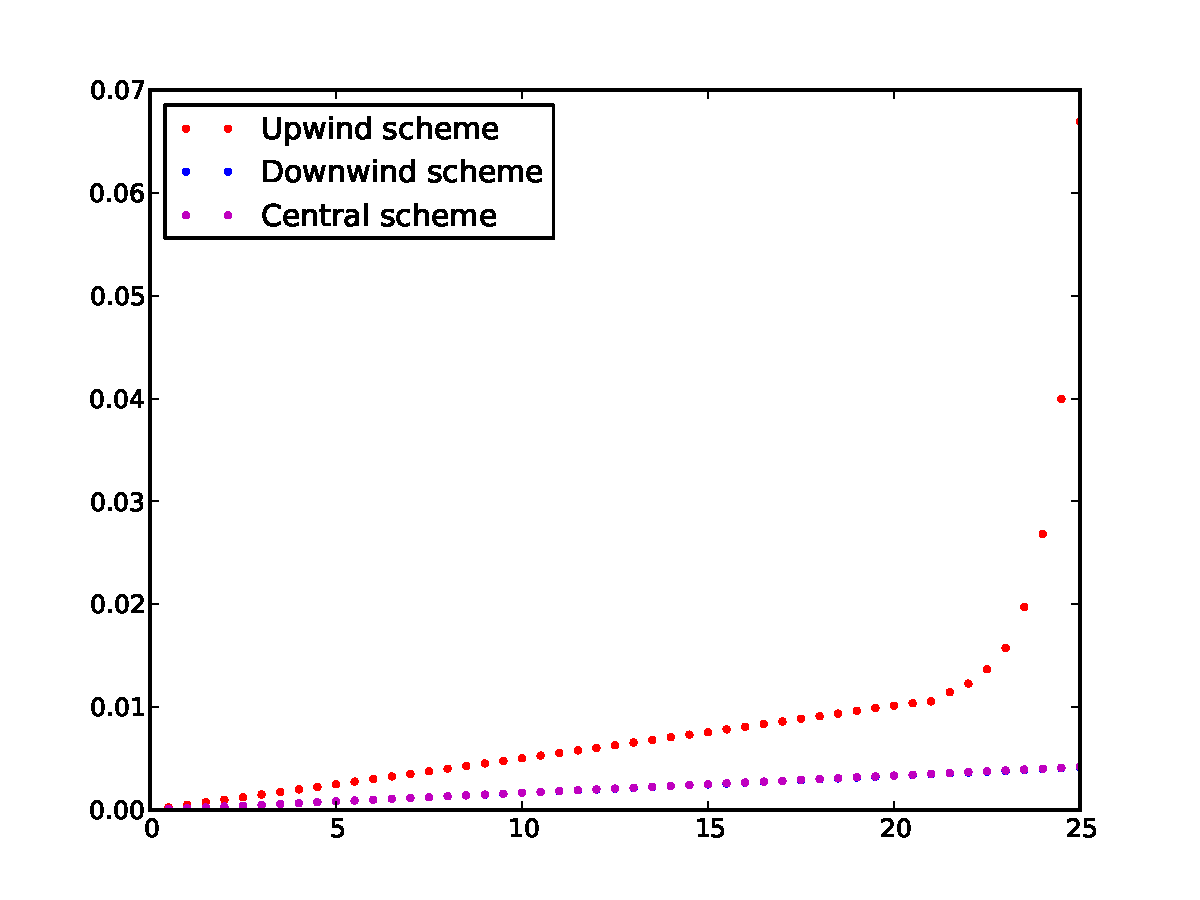
\includegraphics[scale=0.3]{Plots/plot1.pdf}
  \caption{\label{fig:a1} Plot of evolution of relative error through time.}
 \end{center}
\end{figure}

\begin{figure}[hbt]
 \begin{center}
  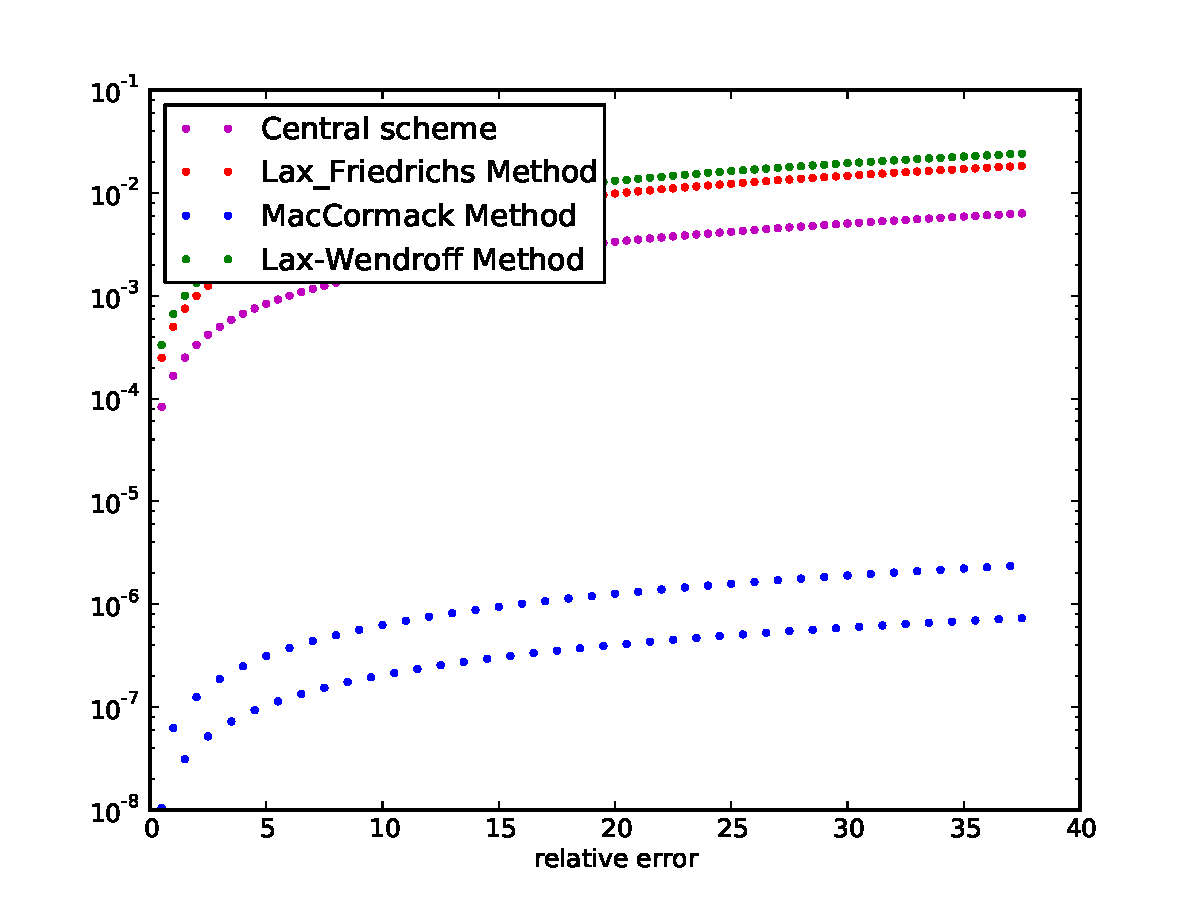
\includegraphics[scale=0.3]{Plots/plot5.pdf}
  \caption{\label{fig:a2} Plot of evolution of relative error through time.}
 \end{center}
\end{figure}

\begin{figure}[hbt]
 \begin{center}
  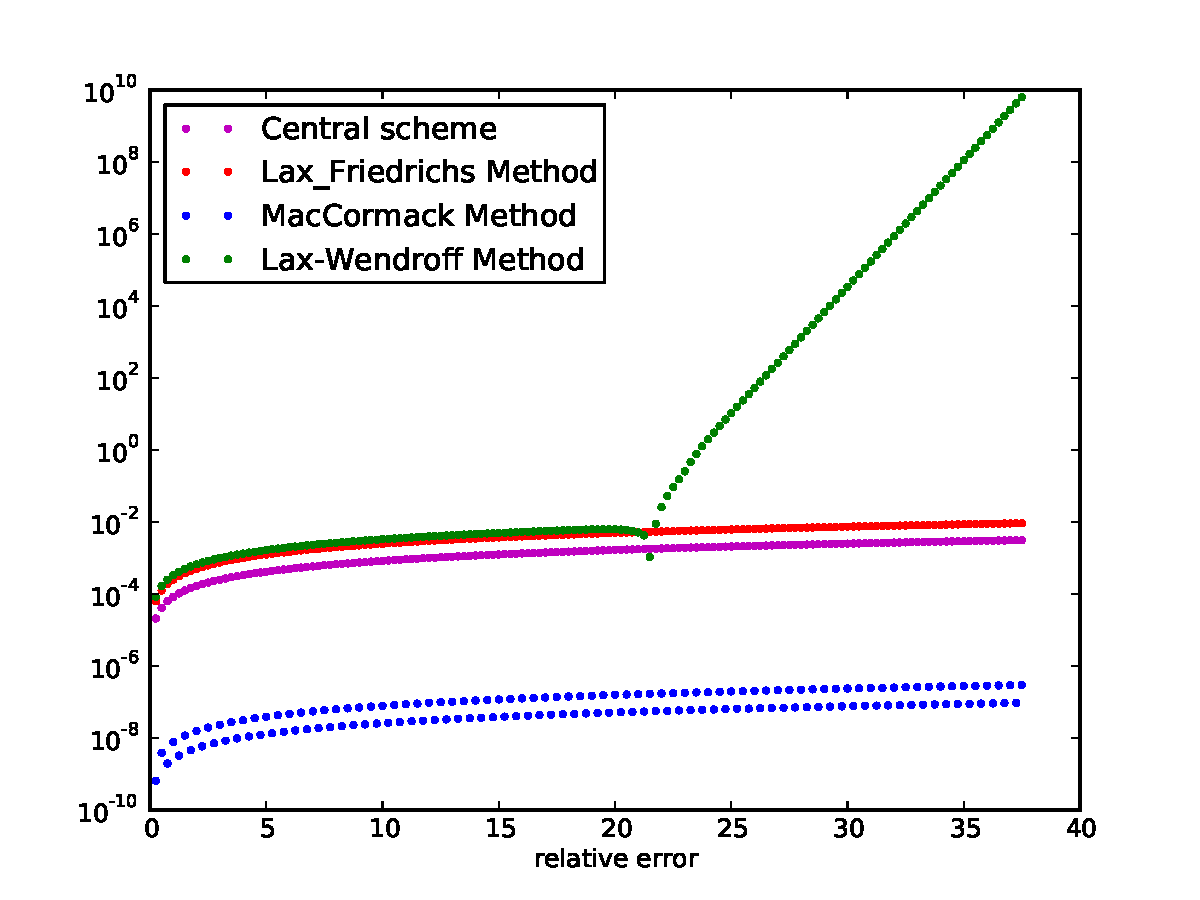
\includegraphics[scale=0.3]{Plots/plot5-2.pdf}
  \caption{\label{fig:a3} Plot of evolution of relative error through time.}
 \end{center}
\end{figure}

Figure \ref{fig:a1} and \ref{fig:a2} and \ref{fig:a3} shows evolution of relative error through time. Based on Figure \ref{fig:a1} it would be obviuse that downwind csheme is not a good method for solving this equation and it is unstable So it is not a good idea to use this method for Advection problem.\\

Also in the next figures I tried to compare several methods such as: central scheme, upwind acheme, Lax-Friedrichs method, MacCormack method, and Lax-Wendroff method. These figures show that MacCormack method is far better than the others and after that Central Scheme is the best one. We can check that Lax-Wendroff method is unstable. And by compareing differeng grid size we can demonstrate that upwind scheme and downwind scheme are firs orther and the other methods are second order.\\

Figure \ref{fig:a2} shows the evolution of relative error for $\delat x = 0.1$ and $\delat t = 0.5$ and figure \ref{fig:a3} shows the evolution of relative error for $\delat x = 0.05$ and $\delat t = 0.25$.\\

\pagebreak




\end{document}
